\documentclass[11pt,letterpaper]{article}
\usepackage{graphicx, geometry, amsmath, hyperref, url, natbib, booktabs, longtable, xcolor, listings}
\geometry{margin=1in}
\hypersetup{colorlinks=true, linkcolor=black, citecolor=black, urlcolor=black}
\renewcommand{\topfraction}{0.9}
\renewcommand{\bottomfraction}{0.8}
\renewcommand{\textfraction}{0.07}
\renewcommand{\floatpagefraction}{0.75}

\title{Newton's Cooling Law Fitted to One Coffee Curve Does Not Transfer Between Cups}
\author{}
\date{}

\begin{document}
\maketitle

\begin{abstract}
Newton's law of cooling is the standard model for hot drinks, but its accuracy for real cups is rarely measured. We fitted Newton's law and a one-term power-law extension to the first 30 minutes of a measured coffee curve in a porcelain pot, froze the constants, and evaluated them on a held-out set of seven published curves from three sources: one coffee cup and six 237 mL cups of hot water. The main result is a paired comparison. Over the held-out set, the power-law extension's mean 30-minute error was 0.19 K lower than Newton's law (paired 95\% interval $-$0.44 to $-$0.00 K). This is one registered in advance criterion, recorded as passed on its sign threshold, but a resampling test gives $p = 0.06$, the advantage reverses when the Manitoba coffee cup is held out, and the set has one coffee curve, so the difference is not established. The accuracy question is answered by the frozen test, which failed: both laws had mean errors near 8 K (Newton's law 8.3 K, 95\% interval 6.5 to 9.9 K) against a registered in advance target of 0.5 K. When the constant was fitted again to the first 10 minutes of each curve, the mean error was 0.64 K over eleven curves, but the one coffee cup stayed at 5.3 K. The scope is one measured coffee curve and no humidity data. A 30-minute accuracy figure for Newton's law describes the cup it was fitted to, not cups in general.
\end{abstract}

\section{Introduction}

Newton's law of cooling says that the rate at which a body loses heat is proportional to its temperature difference from the surroundings. It is the standard model for how a hot drink cools, and it is used in estimates of when a body began cooling. For a cup of coffee, its accuracy over the first half hour is usually stated rather than measured, and the constant that sets the cooling rate is often fitted to the cup being described.

Two questions follow. Published cooling curves for hot drinks are few, and a test of a law on curves it was not fitted to is less common still. Open cups also lose mass and heat by evaporation, which depends on ambient humidity, but the published curves seldom record humidity or cup mass together with the temperature.

We fit Newton's law and a one-term power-law extension to the first 30 minutes of one measured coffee curve, freeze the fitted constants, and evaluate them on curves they never saw. The power-law extension replaces the constant rate with a rate that rises with a power of the temperature difference, and its exponent is fitted along with the rate. We ask two questions: how large is the 30-minute error when the constants are carried to other cups, and whether the fitted exponent is a stable property of cooling or of the one cup it came from. The contributions are:

\begin{itemize}
  \item \textbf{Power-law extension (main result).} Over the held-out set, the power-law extension has a mean 30-minute root-mean-square (RMS) error 0.19 K lower than Newton's law (paired 95\% interval $-$0.44 to $-$0.00 K). This is one registered in advance criterion recorded as passed on its sign threshold. A resampling test gives $p = 0.06$, so the difference is not established, and the advantage reverses when the Manitoba coffee cup is held out.
  \item \textbf{Frozen accuracy.} A frozen Newton law has a mean error of 8.3 K over the seven evaluated curves (95\% interval 6.5 to 9.9 K), against a registered in advance target of under 0.5 K. The frozen test failed; it differs from the target by about an order of magnitude.
  \item \textbf{Exponent.} The in-window exponent is 2.18 (profile 95\% interval 1.95 to 2.42) on the fitting curve. It is a single estimate that was not tested in advance, and it does not carry across cups without fitting again.
  \item \textbf{Fitting to early data.} Fitting the constant again to the first 10 minutes of each held-out cup predicts the remaining 20 minutes with a mean RMS error of 0.64 K over eleven curves. The one coffee cup in that set has an error of 5.3 K. This was not tested in advance, and it rests on one coffee curve and an eight-curve set from three sources.
\end{itemize}

The held-out set is the eight-curve dataset: the fitting curve and seven held-out curves from three sources. The scope is one measured coffee curve, and there are no humidity data or data on a lid or surface cover. Figure~\ref{fig:fig1} sketches the test, and Figure~\ref{fig:fig2} shows the frozen-transfer error for each held-out curve. Section 2 places the work against prior studies, Section 3 gives the data and methods, Section 4 reports the results, and Sections 5 and 6 discuss what the evidence supports and where it stops.

\begin{figure}[!htbp]
  \centering
  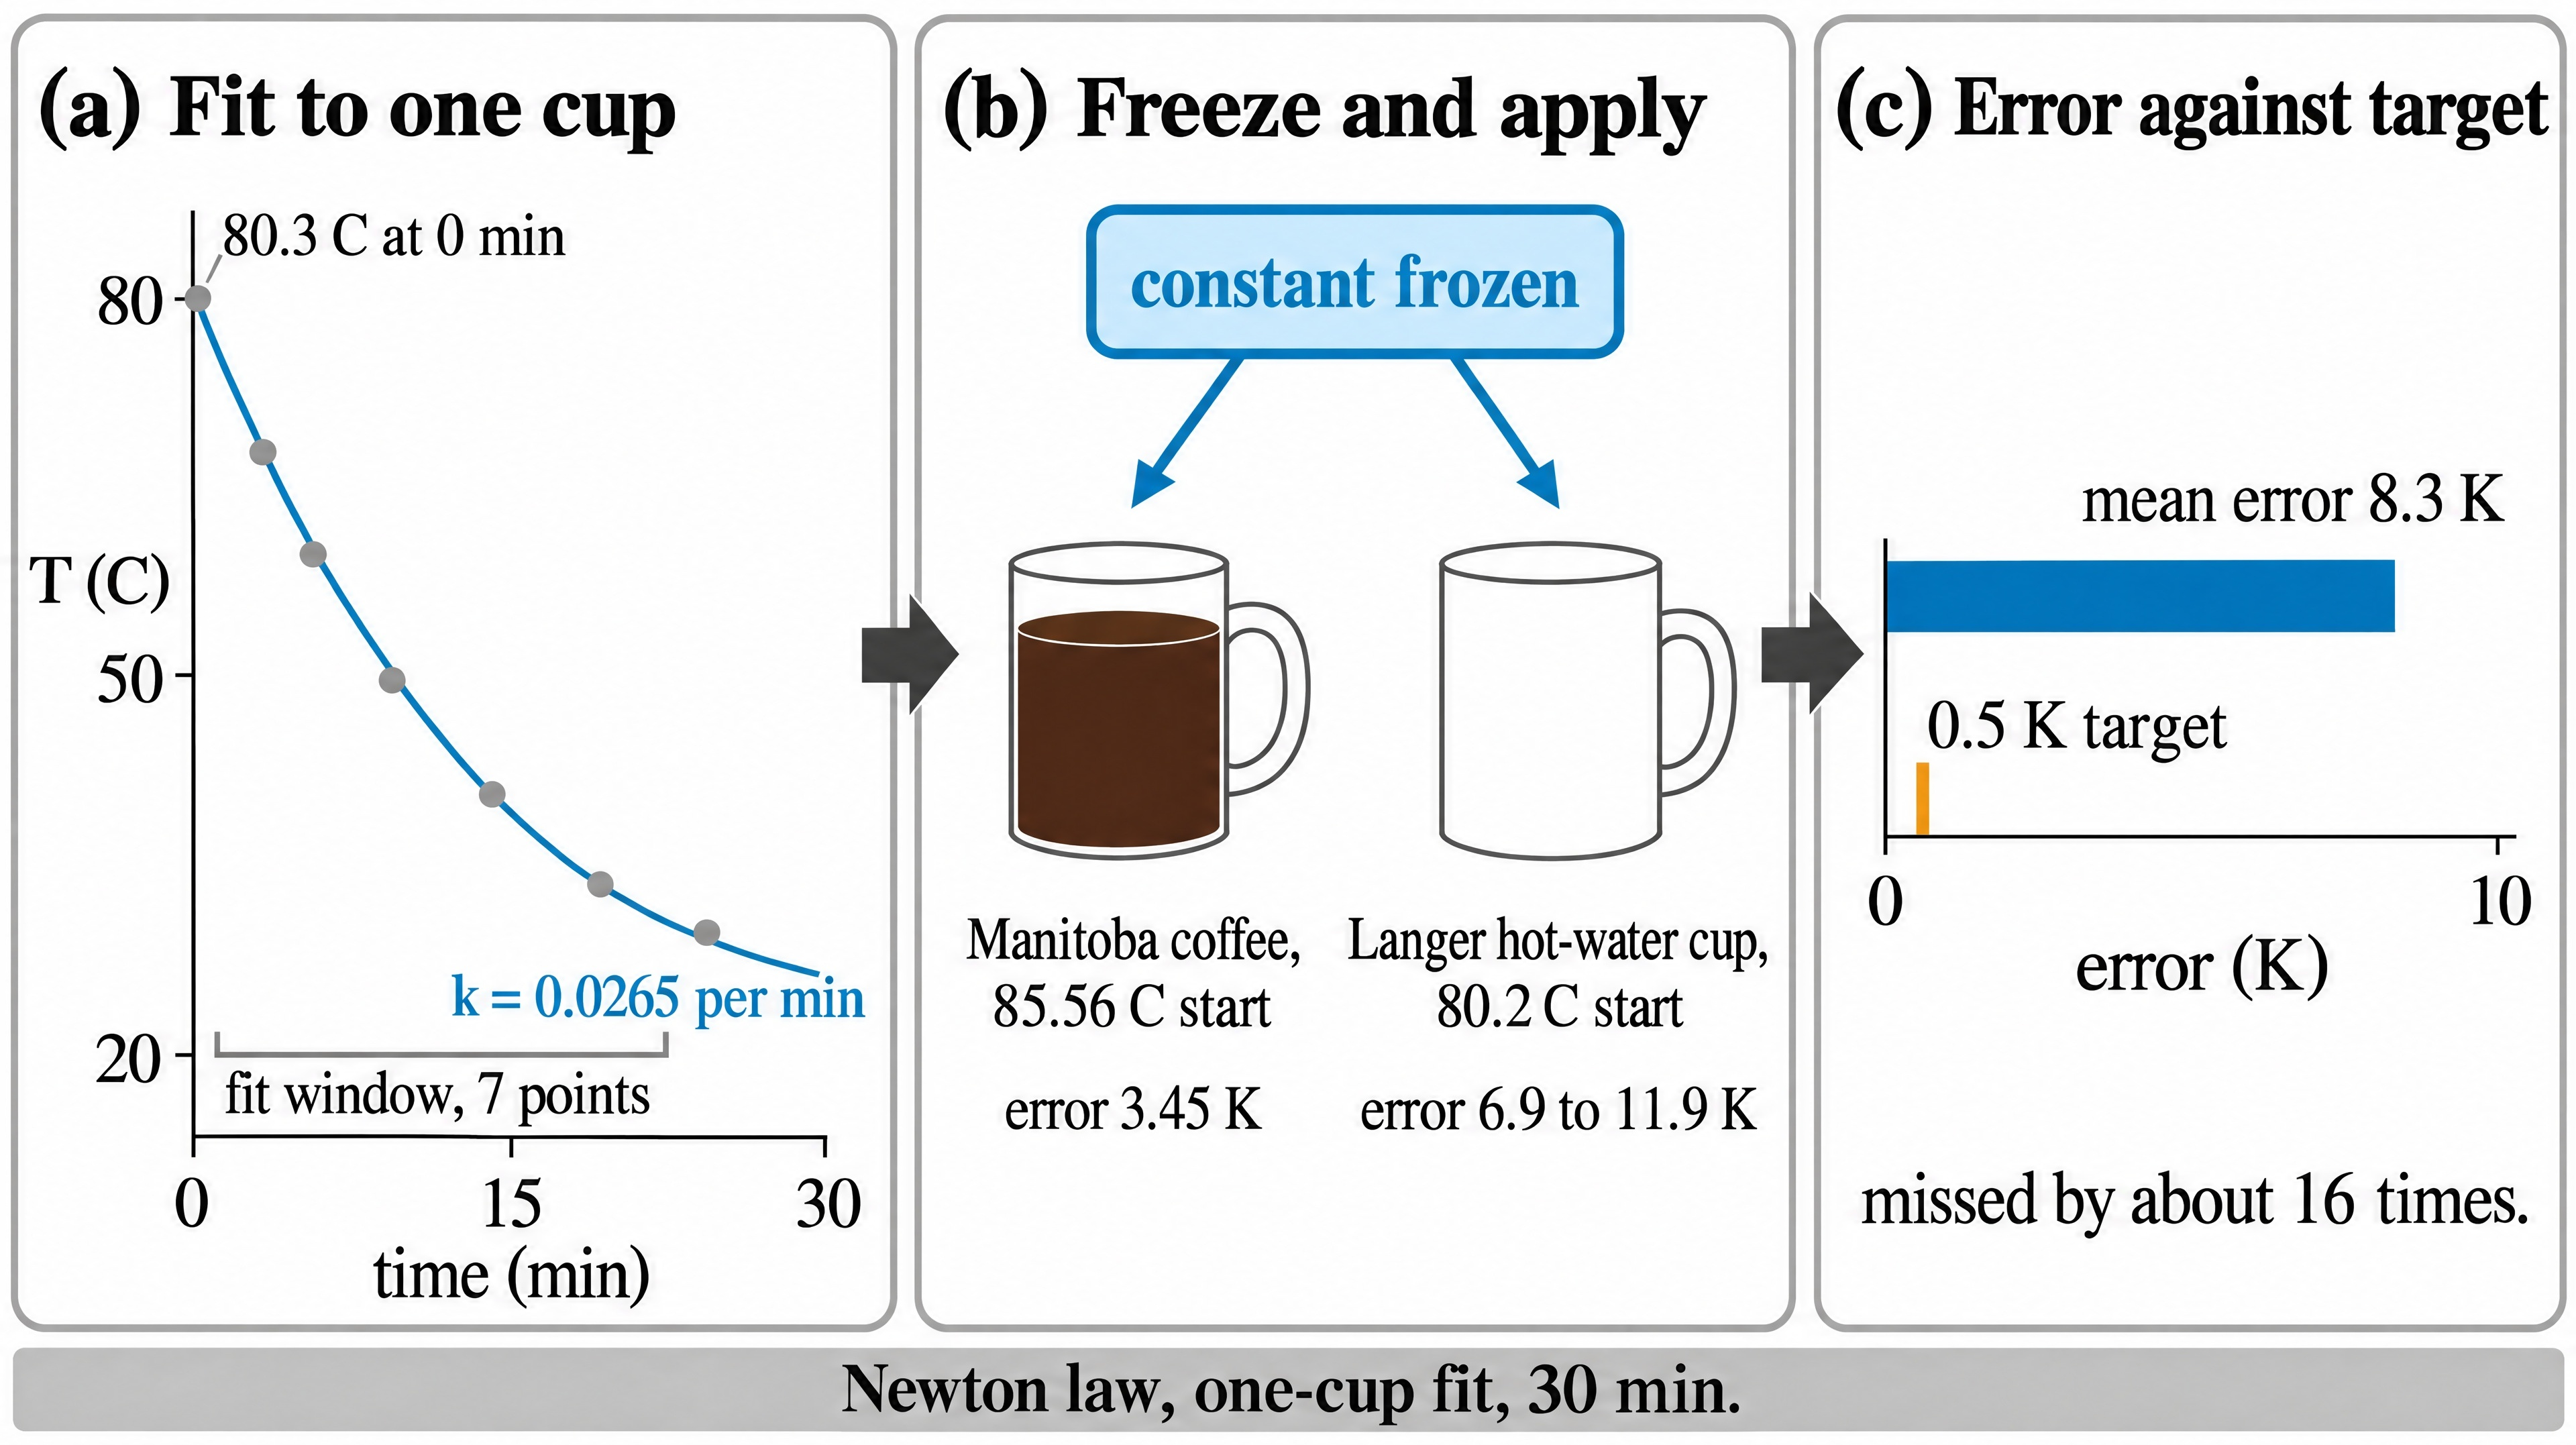
\includegraphics[width=\linewidth,height=0.45\textheight,keepaspectratio]{figures/fig1_v0.jpg}
  \caption{A cooling constant fitted to one cup does not transfer to other cups. The blue Newton-law curve is fitted to the first 30 minutes of a coffee curve measured in a porcelain pot (grey dots) and then frozen; its held-out error is 8.3 K on average, against the 0.5 K target in orange. Schematic illustration of the fit and transfer.}
  \label{fig:fig1}
\end{figure}

\begin{figure}[!htbp]
  \centering
  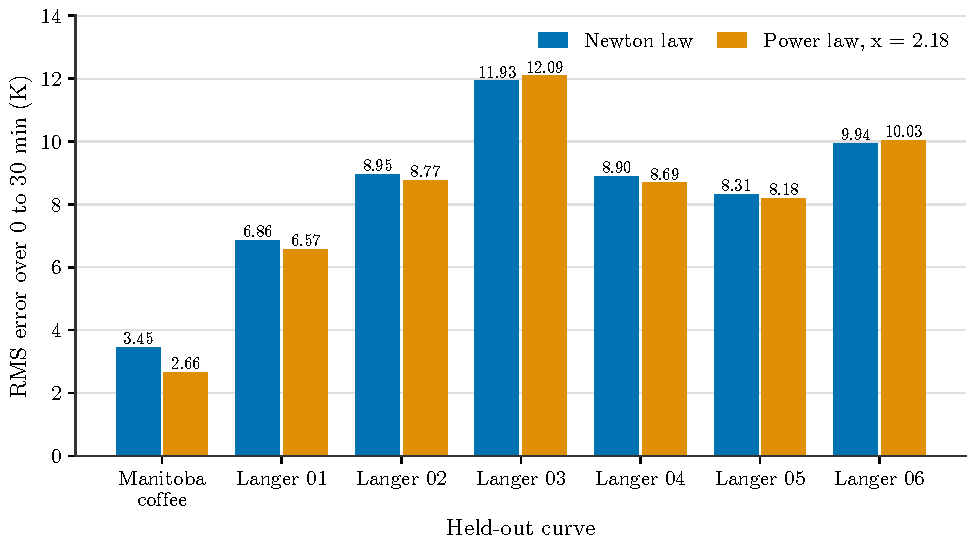
\includegraphics[width=\linewidth,height=0.45\textheight,keepaspectratio]{figures/fig2_v0.pdf}
  \caption{Frozen 30-minute RMS error (K) for each of seven held-out curves, Newton's law (blue) against the power-law extension with $x = 2.18$ (amber). Single-curve values with no intervals. The power law is lower on five of seven curves, and both laws' errors range from 2.7 to 12.1 K.}
  \label{fig:fig2}
\end{figure}

\section{Related Work}

\textbf{Limits of Newton's law.} Vollmer \cite{Vollmer2009} analysed the exponential cooling law and reported that it holds mainly below a temperature-difference threshold that depends on experimental conditions. Above that threshold, radiation, which is not linear in temperature difference, produces significant deviations. The study used solid bodies up to 300 K, not liquids, so it does not give a coffee-cup accuracy figure. This work tests the law on liquids, with its constants carried to cups they were not fitted to. It differs from the threshold analysis in asking how far the error grows when the constant moves between cups, not only when the temperature difference grows.

\textbf{Evaporation and open cups.} A measured coffee curve in a porcelain pot, published by Sedláček and Dolejší, is the curve we fit to. The source reports a fit in which an evaporation term lowers the reduced $\chi^2$ substantially. We could not verify the source's journal, and its reported fit-quality values could not be reproduced from its own drawn curves (Section 3.1). We use only its measured curve. One evaporation-model study, Luniachek et al. (2017), read from its abstract-level summary, uses ambient humidity as a parameter of a theoretical model, not as a variable measured together with a cooling curve. We found no accessible source that records humidity or cup mass with a cooling curve. Several other sources could not be read, so this absence describes what could be read, not the whole literature. This work does not model evaporation, because none of its held-out curves carries humidity data.

\textbf{Published hot-water cup curves.} Langer, Winkler and Lachenmeier (2018) published cooling curves for single-use 237 mL cups of hot water, which we read from figures as six held-out curves. These are the only held-out curves from a source with a different liquid and a different protocol from the fitted curve, and they provide most of the test set.

\section{Method}

\subsection{Data}\label{sec:data}

The data are eight cooling curves from three sources (Table~\ref{tab:data} lists them). The fitting curve is the coffee curve measured in a porcelain pot of Sedláček and Dolejší. It has 29 points from 0 to 138.5 min. We read it from the vector data of the source figure, with axis calibration residuals of 0.06 min in time and 0.21 $^\circ$C in temperature. The source states a thermometer error of 0.3 $^\circ$C, which we use as the reference error. The source reports no ambient temperature, so we use 20 $^\circ$C and note it.

The first held-out curve is a coffee cup on a laboratory table, from the University of Manitoba. It has nine points over 0 to 28 min within the window, a recorded ambient temperature of 21.67 $^\circ$C (71 $^\circ$F), and an initial temperature of 85.56 $^\circ$C. The other six held-out curves are the Langer et al. hot-water cups, read from vector data. Their first recorded temperatures are 80.2 to 82.3 $^\circ$C, not the 88 $^\circ$C serving temperature, and the source reports no ambient temperature. The source's 65 $^\circ$C crossing times, as read from figures, differ from the values the source states (18 to 32 min against 11 to 22 min). We record this discrepancy and use no crossing time in any fit or evaluate.

The source for the fitting curve could not be checked against a Crossref record, and its drawn curves reproduce its stated fit statistics poorly: the ratios of reproduced to reported values fall between 0.03 and 0.29 for the cases we tested. We therefore use the measured points, not the source's statistics.

\subsection{Models}

Newton's law gives the temperature at time $t$ as $T(t) = T_a + (T_0 - T_a)\exp(-k t)$, where $T_0$ is the initial temperature, $T_a$ the ambient temperature and $k$ the cooling rate per minute. The power-law extension replaces the constant rate with a rate that depends on the temperature difference: $dT/dt = -k_c (T - T_a)^x$. Newton's law is the case $x = 1$. The closed-form solution was cross-checked against a numerical solution of the ODE (LSODA) to within $1.6\times10^{-6}$ K on every curve.

\subsection{Fitting and testing protocol}

Both laws are fitted by least squares to the points with $t \le 30$ min on the fitting curve, with 20 random starts; all starts converged. The fitted constants are then frozen. The held-out curves are evaluated by the RMS difference between model and observed temperature over $0 < t \le 30$ min, in kelvin. Residuals are model minus observed, so a positive value means the model is warmer than the liquid.

Ambient temperature is handled in two ways. In ambient A, a recorded ambient temperature is used where one is reported, and 20 $^\circ$C where none is. In ambient B, ambient temperature is a shared parameter fitted within $\pm 5$ K of 20 $^\circ$C. A leave-one-source-out protocol fits again both laws on the other two sources in turn.

\subsection{Uncertainty}

Intervals are bootstrap intervals from 1000 resamples with a fixed random state of 0. For sets of two or more curves, the bootstrap resamples curves. For the single fitting curve, a block bootstrap over time points is used (block length 3), and those intervals are not comparable with between-curve intervals. The paired difference between the two laws is tested with a resampling test, which randomly reverses the sign of each curve's difference and asks how often the mean reaches the observed value.

\subsection{Criteria registered in advance}

Before the held-out curves were evaluated, we fixed four criteria: (i) the power-law extension reaches a held-out 30-minute RMS error under 0.5 K; (ii) it has a lower held-out mean error than Newton's law; (iii) it has the lower error in at least two of the three source folds; (iv) Newton's law predicts the sign of the early residual (0 to 10 min) on the held-out curves. Criterion (i) is the accuracy target, and the 8.3 K main result is assessed against it.

\subsection{Protocol for fitting to early data}

To ask whether the constant transfers once it is allowed to fitted again, we fit each held-out curve on its first 10 minutes and evaluate minutes 10 to 30. For the Manitoba curve the recorded ambient temperature is used. For the Langer cups the ambient temperature is fitted, bounded between $-10$ and 40 $^\circ$C. This protocol was not tested in advance: its exponent was chosen from the fitting curve, and it is tested on the same held-out curves.

\section{Results}

\subsection{Fit to the measured coffee curve}\label{sec:fit}

On the fitting curve, Newton's law has an in-window RMS error of 1.26 K (block-bootstrap interval 0.94 to 1.37 K). The power-law extension has an RMS error of 0.33 K (0.05 to 0.46 K) with an exponent of 2.18 and $k_c = 2.82\times10^{-4}$ per minute. The errors have a clear shape. Newton's law runs warm by a mean of 1.03 K over the first 10 minutes and cool by 0.45 K over minutes 10 to 30 (model minus observed). The power-law extension removes most of this pattern. These are in-sample values: they describe how well each law fits the curve it was fitted to, and they say nothing about other cups.

\subsection{Frozen transfer to held-out curves}\label{sec:frozen}

Table~\ref{tab:frozen} gives the frozen-transfer results under ambient A. The per-curve values are in Table~\ref{tab:a2} and Figure~\ref{fig:fig2}.

\begin{table}[!htbp]
  \centering
  \caption{Frozen 30-minute RMS error (K) on the seven evaluated curves of the held-out set under ambient A. Intervals are 95\% bootstrap over curves.}
  \label{tab:frozen}
  \begin{tabular}{lccc}
    \toprule
    Set & Curves & Newton law & Power law ($x = 2.18$) \\
    \midrule
    Manitoba coffee & 1 & 3.45 & 2.66 \\
    Langer hot-water cups & 6 & 9.15 & 9.06 \\
    All held-out curves & 7 & 8.33 (6.54 to 9.93) & 8.14 (5.93 to 9.96) \\
    \bottomrule
  \end{tabular}
\end{table}

This is the main result. On the seven evaluated curves, the power-law extension has the lower mean error, with a paired difference of $-0.19$ K (95\% interval $-0.44$ to $-0.00$ K) and a lower error on five of seven curves. The criterion's threshold is a lower mean for the power law, and it is recorded as passed on that threshold. The resampling test gives $p = 0.0625$ for the mean difference and $p = 0.23$ for the count, so the advantage is not established on this set (Figure~\ref{fig:fig2}). Under ambient B the means are 8.25 K and 8.03 K, and the conclusions do not change.

The accuracy target fails, and this is the result of the frozen test. Neither law comes near 0.5 K on the Manitoba coffee cup or on the Langer cups, and the mean error of 8.3 K is the main result of this study. Table~\ref{tab:criteria} gives all four criteria.

\begin{table}[!htbp]
  \centering
  \caption{Criteria registered in advance and outcomes, ambient A.}
  \label{tab:criteria}
  \begin{tabular}{p{0.36\linewidth}p{0.33\linewidth}p{0.21\linewidth}}
    \toprule
    Criterion & Observed & Outcome \\
    \midrule
    (i) Power-law held-out RMS under 0.5 K & Manitoba 2.66 K; Langer mean 9.06 K & Failed \\
    (ii) Power law lower on held-out mean (threshold: any negative mean difference) & $-0.19$ K; lower on 5 of 7 curves & Passed on the sign threshold; resampling $p = 0.0625$ beside it \\
    (iii) Power law lower in at least 2 of 3 folds & Lower on the fitting-source and Langer folds; higher on Manitoba & Passed \\
    (iv) Newton law early residual positive & Mean $-3.20$ K over 0 to 10 min; positive on 1 of 7 curves & Failed \\
    \bottomrule
  \end{tabular}
\end{table}

The early residual fails because the errors have opposite signs on the two sets. On the Manitoba coffee cup, Newton's law runs warm by 2 to 5 K at every point in the window, so the observed cup cools faster than the fitted constant predicts. On the Langer cups it runs cold over the first 10 minutes, so the fitted constant predicts more heat loss than those cups show. A single constant therefore is off in opposite directions on the two sets.

The leave-one-source-out fits show the same instability, and this limits the main comparison. When the Langer cups are held out and both laws are fitted again on the other two sources, the power law is lower on all six cups (mean difference $-0.50$ K). When the Manitoba coffee cup is held out, its fit reverses the sign. The advantage of the power-law extension therefore depends on which source is held out.

\subsection{Stability of the exponent}\label{sec:exponent}

The in-window exponent is 2.18. Profiling the in-window fit over the exponent gives a minimum at $x = 2.18$ with a $\Delta\chi^2 = 3.84$ interval of 1.95 to 2.42 ($\sigma = 0.3$ K). A 200-replicate moving-block bootstrap of the residuals gives a median of 2.21 and a 95\% interval of 2.03 to 2.36. A first search range that ended at $x = 2.00$ had its minimum at that edge, so we extended the range to 3.00 before reporting. Under strict transfer, where the exponent and rate are carried over as fixed values, only the Manitoba curve can be evaluated, because the Langer cups report no ambient temperature. There the frozen Newton law has an error of 3.66 K and the frozen power law an error of 2.82 K. The 3.66 K differs from the 3.45 K in Table~\ref{tab:frozen} because this analysis omits the $t = 0$ point.

\subsection{Fitting again to the first 10 minutes}\label{sec:fitted again}

When each held-out curve's constant is fitted again to its first 10 minutes and tested over minutes 10 to 30 (Figure~\ref{fig:fig3}), the mean RMS error over eleven curves is 0.64 K for Newton's law and 0.60 K for the power law at $x = 2.18$. The eleven are the Manitoba cup and all ten read from figures Langer cups; four of the Langer cups lie outside the planned set of six (Appendix A), so this is a wider test than the frozen one. The mean is carried by the Manitoba coffee cup, where the Newton law has an error of 5.30 K and the power law of 0.77 K. On the ten Langer cups, Newton's law has a mean error of 0.18 K, and every cup lies below 0.3 K. The power law is better on two of the eleven curves and worse on nine of the ten Langer cups. In this fitted again the exponent adds no accuracy, and a constant fitted again to early data predicts the Langer cups well while the coffee cup stays poorly predicted.

\begin{figure}[!htbp]
  \centering
  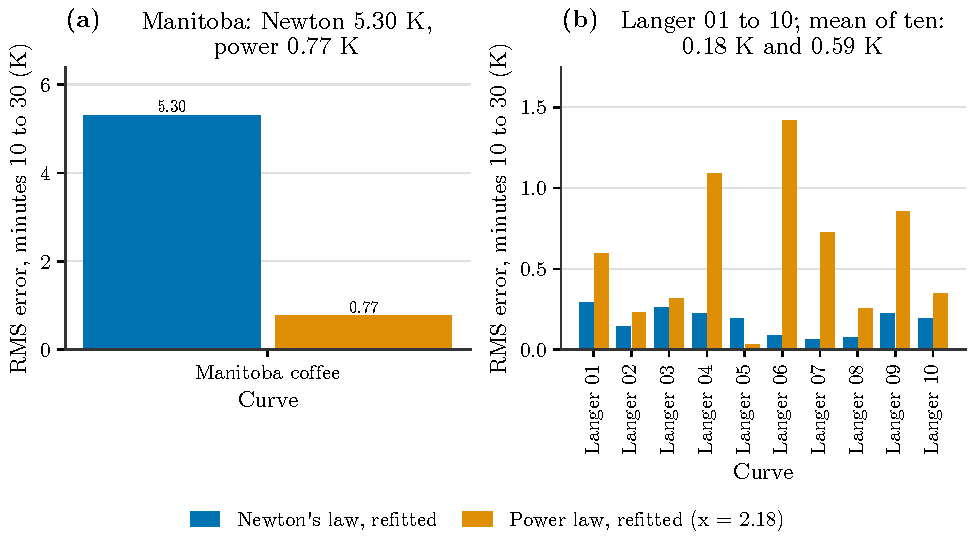
\includegraphics[width=\linewidth,height=0.45\textheight,keepaspectratio]{figures/fig3_v0.pdf}
  \caption{RMS error over minutes 10 to 30 after fitting again, each curve fitted again to its first 10 minutes. Newton's law (blue) is worst on the Manitoba coffee cup, 5.30 K; the power law (amber, $x = 2.18$) is lower on two of eleven curves, Manitoba and Langer 05. The ten Langer cups are read from figures curves outside the planned set.}
  \label{fig:fig3}
\end{figure}

\section{Discussion}

The main finding is that a Newton-law constant fitted to one cup does not predict the 30-minute temperature of other cups within half a kelvin. The frozen error is about 8 K on average, and the power-law extension changes it by 0.19 K, a difference the resampling test does not establish. The fitted again result shows the other side: the law's accuracy is a property of the cup and its fitted again, not of the law. A reported 30-minute accuracy figure for Newton's law on a drink should therefore name the cup it was fitted to, the window, and whether the constant was fitted again, and it should be checked on a cup whose data were not used in the fit.

The exponent should not be read as a physical constant. It is fitted to about seven points from one cup. It may absorb evaporation, heat loss to the surface, or the shape of the cup, and the held-out curves carry no humidity data or data on a lid or surface cover that could separate these. Its stability across the fitting window and bootstrap samples is a statement about that window, not about cups in general.

For those who build and test cooling models, the testing implication is that a held-out cup set with a frozen constant is a strict test that a single in-sample fit cannot pass. A model that fits its own curve to 0.3 K can still be 8 K wrong for a second cup. Tests should report transfer error across cups together with in-sample error, and should record the ambient temperature and humidity that a model needs.

\section{Limitations}

\begin{itemize}
  \item \textbf{Scope of the evidence.} The fitting curve is one measured coffee curve in a porcelain pot. The held-out set has eight curves from three sources, and six of the eight are hot-water cups from one lab and protocol, so they are not six independent measurements. Only one held-out curve is coffee.
  \item \textbf{Missing variables.} No source reports relative humidity, and no source reports a lid or surface cover, so evaporation and the effect of a lid or surface cover are not tested. The metal and vacuum pot curves are not published as data and could not be used.
  \item \textbf{Ambient temperature.} The ambient temperature was not reported for the fitting curve or for the Langer cups, and 20 $^\circ$C is an assumption. Moving from ambient A to ambient B changes the Manitoba error by 0.6 K for Newton's law and by 0.8 K for the power law. The cause of this shift is not isolated.
  \item \textbf{Parameter bounds.} Several fits again end on parameter bounds. Four of the ten Langer fits again in Section~\ref{sec:fitted again} reach the $-10$ $^\circ$C lower bound of the ambient search, and two more fitted ambient temperatures are outside a plausible range for a room, as noted in the outputs. These fits reduce confidence in the fit-again errors for those cups.
  \item \textbf{Agreement with published values.} Our reading of the fitting curve from its figure did not reproduce the fit statistics the source reports. A first reading gave an in-window error of 1.07 K for Newton's law, and a second reading from the same data read from figures gave 1.26 K. The cause is open, and the 1.26 K value is used throughout. The exponent in the first reading was 1.94, against 2.18 in the second.
  \item \textbf{Reading from figures.} The Langer curves and the fitting curve were read from figures. The fitting curve's reading discrepancy across four repeated figures has a median of 0.15 K, and the Langer crossing times differ from the source's stated values. Errors from reading the figures are small compared with the 8 K main result but not compared with the 0.3 K fit-again errors.
  \item \textbf{Sensitivity.} Four further Langer curves were read from figures but kept out of the planned set. Evaluating all ten with the frozen parameters gives a mean error of 9.17 K for Newton's law and 9.05 K for the power law, so the planned set does not drive the result.
  \item \textbf{Reference records.} The journal of the fitting-curve study and the Crossref record of the Langer et al. study could not be verified against a Crossref or Semantic Scholar record. They are cited by author and year only.
\end{itemize}

\section{Conclusion}

Newton's law of cooling, with a constant fitted to one measured coffee cup, did not predict the 30-minute temperatures of seven other curves within the 0.5 K target. Its frozen mean error is 8.3 K (95\% interval 6.5 to 9.9 K), and a power-law extension changes that by 0.19 K, a difference the resampling test does not establish. When the constant is fitted again on the first 10 minutes, the mean error is 0.64 K over eleven curves, but the one coffee cup in the set remains at 5.3 K. Future tests should use more coffee curves recorded with humidity and cup mass, and should report transfer error across cups as the main accuracy figure.

\section*{Code availability}

Code, prompts, raw outputs and the programs that reproduce each number are in the paper's code archive~\href{https://github.com/ai-inventor-papers/ai-invention-5821c4-newtons-cooling-law-for-coffee-over-30/tree/main}{[code]}, and Appendix~\ref{app:code} links each result to the code archive that produced it.

\bibliographystyle{unsrt}
\bibliography{references}

\clearpage
\appendix

\section{Data and tasks}\label{app:data}

\begin{table}[!htbp]
  \centering
  \caption{The eight curves.}
  \label{tab:data}
  \begin{tabular}{p{0.22\linewidth}p{0.22\linewidth}p{0.20\linewidth}p{0.13\linewidth}p{0.19\linewidth}}
    \toprule
    Curve & Source & Liquid and vessel & Initial temp. ($^\circ$C) & Ambient temp. ($^\circ$C) \\
    \midrule
    Sedláček and Dolejší & Sedláček and Dolejší & Coffee, porcelain pot & 80.25 & 20 (assumed) \\
    Manitoba coffee & University of Manitoba laboratory & Coffee, laboratory table & 85.56 & 21.67 (recorded) \\
    Langer 01 to 06 & Langer et al. (2018) & Hot water, 237 mL cup & 80.2 to 82.3 & 20 (assumed) \\
    \bottomrule
  \end{tabular}
\end{table}

\textbf{Task.} The model is given an initial temperature, an ambient temperature where one is recorded, and the cooling time, and it must return the liquid temperature at each later time. Its output is evaluated against the measured temperature read from the figures at each point with $0 < t \le 30$ min. An example record is the Manitoba curve: initial temperature 85.56 $^\circ$C, ambient temperature 21.67 $^\circ$C, nine measured points over 0 to 28 min. The error is the RMS of model minus observed over those points, in kelvin; lower is better. A curve counts as ``correct'' against the 0.5 K target if its error is below 0.5 K.

\begin{table}[!htbp]
  \centering
  \caption{Per-curve 30-minute RMS error (K), ambient A, frozen parameters.}
  \label{tab:a2}
  \begin{tabular}{lcc}
    \toprule
    Curve & Newton law & Power law ($x = 2.18$) \\
    \midrule
    Manitoba coffee & 3.45 & 2.66 \\
    Langer 01 & 6.86 & 6.57 \\
    Langer 02 & 8.95 & 8.77 \\
    Langer 03 & 11.93 & 12.09 \\
    Langer 04 & 8.90 & 8.69 \\
    Langer 05 & 8.31 & 8.18 \\
    Langer 06 & 9.94 & 10.03 \\
    \bottomrule
  \end{tabular}
\end{table}

\begin{table}[!htbp]
  \centering
  \caption{Fitting again to the first 10 minutes, tested over minutes 10 to 30 (K).}
  \label{tab:a3}
  \begin{tabular}{lcc}
    \toprule
    Curve & Newton law & Power law ($x = 2.18$) \\
    \midrule
    Manitoba coffee & 5.30 & 0.77 \\
    Langer 01 & 0.29 & 0.60 \\
    Langer 02 & 0.15 & 0.23 \\
    Langer 03 & 0.26 & 0.32 \\
    Langer 04 & 0.22 & 1.09 \\
    Langer 05 & 0.19 & 0.03 \\
    Langer 06 & 0.09 & 1.42 \\
    Langer 07 & 0.06 & 0.72 \\
    Langer 08 & 0.08 & 0.25 \\
    Langer 09 & 0.23 & 0.85 \\
    Langer 10 & 0.19 & 0.35 \\
    \bottomrule
  \end{tabular}
\end{table}

\textbf{Sensitivity check.} All ten read from figures Langer curves, evaluated with the frozen planned parameters: Newton law 9.17 K, power law 9.05 K.

\section{Code for each result}\label{app:code}

Each row links the code archive, on the run's code branch, of the experiment behind a result.

\begin{longtable}{p{0.22\linewidth}p{0.38\linewidth}p{0.32\linewidth}}
  \toprule
  Section & Result & Code archive \\
  \midrule
  \endhead
  \S\ref{sec:data} & Digitized fitting curve and reproduction of its fit statistics & \href{https://github.com/ai-inventor-papers/ai-invention-5821c4-newtons-cooling-law-for-coffee-over-30/tree/main/round-1/experiment-1}{\texttt{round-1/experiment-1}} \\
  \S\ref{sec:frozen} & Frozen transfer, main comparison (Table~\ref{tab:frozen}, Figure~\ref{fig:fig2}) & \href{https://github.com/ai-inventor-papers/ai-invention-5821c4-newtons-cooling-law-for-coffee-over-30/tree/main/round-2/experiment-2}{\texttt{round-2/experiment-2}} \\
  \S\ref{sec:exponent} & Stability of the exponent (profile and bootstrap) & \href{https://github.com/ai-inventor-papers/ai-invention-5821c4-newtons-cooling-law-for-coffee-over-30/tree/main/round-2/experiment-3}{\texttt{round-2/experiment-3}} \\
  \S\ref{sec:fit} & Fit of Newton's law and the power-law extension to the fitting curve (Section~\ref{sec:fit}) & \href{https://github.com/ai-inventor-papers/ai-invention-5821c4-newtons-cooling-law-for-coffee-over-30/tree/main/round-1/experiment-1}{\texttt{round-1/experiment-1}} \\
  \S\ref{sec:fitted again} & Fitting again to the first 10 minutes, tested over minutes 10 to 30 (Figure~\ref{fig:fig3}) & \href{https://github.com/ai-inventor-papers/ai-invention-5821c4-newtons-cooling-law-for-coffee-over-30/tree/main/round-2/experiment-2}{\texttt{round-2/experiment-2}} \\
  App.~\ref{app:data} & The eight curves (Table~\ref{tab:data}) & \href{https://github.com/ai-inventor-papers/ai-invention-5821c4-newtons-cooling-law-for-coffee-over-30/tree/main/round-1/dataset-1}{\texttt{round-1/dataset-1}}, \href{https://github.com/ai-inventor-papers/ai-invention-5821c4-newtons-cooling-law-for-coffee-over-30/tree/main/round-2/dataset-2}{\texttt{round-2/dataset-2}} \\
  Section~1 & Power-law extension, main paired comparison & \href{https://github.com/ai-inventor-papers/ai-invention-5821c4-newtons-cooling-law-for-coffee-over-30/tree/main/round-2/experiment-2}{\texttt{round-2/experiment-2}} \\
  Section~1 & Exponent 2.18 on the fitting curve & \href{https://github.com/ai-inventor-papers/ai-invention-5821c4-newtons-cooling-law-for-coffee-over-30/tree/main/round-2/experiment-3}{\texttt{round-2/experiment-3}} \\
  Section~2 & Evaporation and humidity literature check & \href{https://github.com/ai-inventor-papers/ai-invention-5821c4-newtons-cooling-law-for-coffee-over-30/tree/main/round-1/research-1}{\texttt{round-1/research-1}} \\
  Section~3.1 & Fitting-curve reading from figures and reproduction check & \href{https://github.com/ai-inventor-papers/ai-invention-5821c4-newtons-cooling-law-for-coffee-over-30/tree/main/round-1/experiment-1}{\texttt{round-1/experiment-1}} \\
  \bottomrule
\end{longtable}

\end{document}
